\chapter{Resultaten met de custom  modellen}
\label{ch:resultaten-custom-model}

In ongeveer een kwartier tijd hebben zowel het periodemodel als het themamodel de 845 beelden van Huis van Alijn ingedeeld periodes of thema’s. In die 845 beelden zaten ook de beelden die gebruikt werden voor training en validatie. Het was opmerkelijk om vast te stellen dat ook deze beelden soms door de modellen fout geclassificeerd werden. Clarifai gaf meerdere tags per foto. Omdat een foto slechts ingedeeld kan worden in één thema, hielden we enkel rekening met de tag die de hoogste waarschijnlijkheidsscore gekregen heeft.

In dit hoofdstuk worden afzonderlijk de resultaten van beide modellen besproken. Tot slot zal net als in hoofdstuk \ref{ch:resultaten-ingebouwd-model} suggesties gedaan worden voor de toepassing in de praktijk.  

\section{Themamodel}
\label{sec:themamodel}

Het Themamodel heeft 845 beelden geanalyseerd en geclassificeerd. 753 beelden (89\%) werden correct geclassificeerd.  De waarschijnlijkheidsscore van de tags bevond zich tussen 100\% en 39\% en had een gemiddelde van 94,6\%. De gemiddelde rappel voor de vijf thema’s is 90\%, terwijl de gemiddelde precisie een waarde van 86\% heeft.

\begin{table}
	\centering
     \renewcommand\arraystretch{1.2}
    \begin{tabular}{l|ccc|rrr}
        \toprule
         & true positives  & false negatives & false positives & rappel & precisie & $F_1$-score \\
        \midrule
        geboorte & 81 & 15 & 50 & 84\% & 62\% & 71\% \\
        huwelijk & 346 & 54 & 6 & 87\% & 98\% & 92\% \\
        Sint & 93 & 4 & 1 & 96\% & 99\% & 97\% \\
        speelgoed & 88 & 13 & 21 & 87\% & 81\% & 84\% \\
        vakantie & 145 & 6 & 14 & 96\% & 91\% & 94\% \\
        \midrule
        gemiddelde & 150,6 & 18,4 & 18,4 & 90\% & 86\% & 88\% \\
        \bottomrule
    \end{tabular}
    \caption{De performantie (rappel, precisie en $F_1$-score) van het Themamodel op de volledige dataset van Huis van Alijn.}
    \label{tab:resultaten-themamodel}
\end{table}

Het custom model kon de foto's van het thema Sinterklaas het beste indelen ($F_1$-score van 97\%). Dit thema haalde in hoofstuk \ref{ch:resultaten-ingebouwd-model} nog de slechtste resultaten, maar heeft bij het Themamodel de grootste precisie en de tweede grootste rappel. Dit is te verklaren doordat de foto’s sterk op elkaar lijken. Op iedere foto staat een oudere man met baard en mijter, vergezeld door een of meerdere kinderen die met de oude man op de foto poseren. Opvallend is ook de sterke score van de vakantiefoto’s ($F_1$-score van 94\%), terwijl deze foto’s juist gekenmerkt worden door een grote variëteit (strandfoto’s, kampeerfoto’s, citytrips, wintersport,...).

Het model scoorde het minst op geboortefoto’s. Vooral de precisie voor deze foto’s zijn ondermaats (62\%). Er waren vijftig false positives\footnote{Dit zijn vijftig foto's die foutief het label geboorte kregen.}. Veel huwelijksfoto’s (54 false negatives\footnote{~Dit zijn 54 huwelijksfoto's die niet als huwelijksfoto herkend werden.}) werden immers als geboortefoto herkend.  Net als in vorig hoofdstuk waren de resultaten met de speelgoedfoto’s niet zo goed. Zowel de precisie als de rappel zijn lager dan het gemiddelde.

Lagere scores zijn soms te wijten aan de vaag afgebakende thema’s door het museum. Sommige foto’s die door het museum ingedeeld werden in het thema Speelgoed zijn foto’s van kinderen met een stuk speelgoed op vakantie, terwijl er ook vakantiefoto’s zijn waar kinderen met speelgoed op poseren. Dit verklaart waarom het model zeven speelgoedfoto’s classificeert als vakantiefoto’s en vier vakantiefoto’s als speelgoedfoto. Het model had het ook moeilijk om poppen van baby’s te onderscheiden. Negen geboortefoto’s werden door het model ingedeeld in het thema Speelgoed, terwijl zes speelgoedfoto’s als geboortefoto beschouwd werden (zie tabel \ref{tab:confusion-matrix-themamodel}).

\begin{figure}
	\centering
	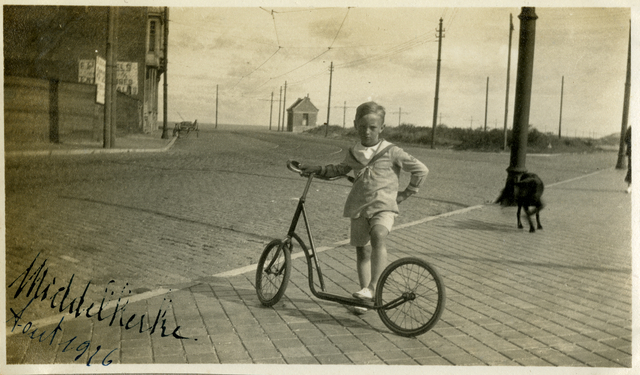
\includegraphics[width=\textwidth]{FO-20-00098.jpg}\hfill
	\\[\smallskipamount]
	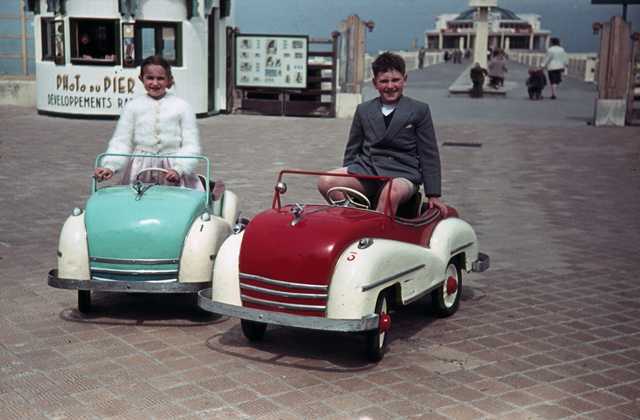
\includegraphics[width=\textwidth]{DIA-0037-0149.jpg}\hfill
	\caption[Voorbeeld van foto's van de thema's Vakantie en Speelgoed die gelijkend zijn]{Voorbeeld van foto's van de thema's Vakantie en Speelgoed die gelijkend zijn. De bovenste foto is een foto die door Huis van Alijn ingedeeld werd in het thema Speelgoed, de onderste foto is een vakantiefoto.}
\end{figure}

Zoals in hoofdstuk \ref{ch:resultaten-ingebouwd-model} werd geanalyseerd of het model slechter scoort op foto’s uit vroegere periodes. Dit lijkt niet het geval te zijn. Foto’s uit de jaren 60 (en 50) hebben een grotere foutenmarge, maar dit valt te verklaren door de grote hoeveelheid huwelijksfoto’s uit deze periode.

\begin{table}
    \centering
    \renewcommand\arraystretch{1.2}
    \settowidth\rotheadsize{\theadfont Feitelijk thema}   
    \begin{tabular}{@{} cc | cccccc}
        \toprule
        &  & & \multicolumn{5}{c}{\textbf{Voorspeld thema}}  \\
        &  & & geboorte & huwelijk & sint & speelgoed &  vakantie  \\
        \midrule
        \multirow{5}{*}[1ex]{\rothead {\textbf{Feitelijk thema}}}
        & geboorte   &  &  \cellcolor{hgpink}81 & 3 & 1 & 9 & 2 \\
        & huwelijk  &   & 43 & \cellcolor{hgpink}346 & 0 & 6 & 5 \\
        & sint  &   & 1 & 1 & \cellcolor{hgpink}93 & 2 & 0 \\
        & speelgoed  &  & 6 & 0 & 0 & \cellcolor{hgpink}88 & 7 \\
        & vakantie & & 0 & 2 & 0 & 4 & \cellcolor{hgpink}145 \\
        \bottomrule
    \end{tabular}
    \caption[Confusion matrix voor het Themamodel.]{Confusion matrix voor het Themamodel. Het Themamodel slaagt erin om meestal het juiste thema eruit te halen.}
    \label{tab:confusion-matrix-themamodel}
\end{table}

\section{Periodemodel}
\label{sec:periodemodel}

Ook het Periodemodel heeft 845 beelden geanalyseerd en geclassificeerd. Omdat van 42 beelden de periode niet gekend was door het museum en we dus niet konden nagaan of het model ze juist geclassificeerd heeft, werden deze beelden niet meegerekend bij de beoordeling van de resultaten. 

Het model had 460 beelden (57\%) correct geclassificeerd. De waarschijnlijkheidsscore van de tags bevond zich tussen 94\% en 20\% en had een gemiddelde van slechts 55\%. Dit kan betekenen dat het model ofwel te weinig trainingsbeelden had om de verschillende concepten te kunnen onderscheiden, of dat de taak te moeilijk is voor een CV API. De gemiddelde rappel voor de tien periodes is maar 57\%, terwijl de gemiddelde precisie een waarde van 62\% heeft.

\begin{table}
	\centering
    \renewcommand\arraystretch{1.2}
    \begin{tabular}{l|ccc|rrr}
        \toprule
        & true positives  & false negatives & false positives & rappel & precisie & $F_1$-score \\ 
        \midrule
        00s & 3 & 6 & 0 & 33\% & 100\% & 50\% \\ 
        10s & 13 & 3 & 8 &  81\% & 62\% & 70\% \\ 
        20s & 14 & 18 & 15 & 44\% & 48\% & 46\% \\ 
        30s & 34 & 20 & 45  & 63\% & 43\% & 51\% \\ 
        40s & 40 & 21 & 70  & 66\% & 36\% & 47\% \\ 
        50s & 110 & 99 & 71  & 53\% & 61\% & 56\% \\ 
        60s & 120 & 106 & 56  & 53\% & 68\% & 60\% \\ 
        70s & 73 & 41 & 51  & 64\% & 59\% & 61\% \\ 
        80s & 43 & 18 & 24  & 71\% & 64\% & 67\% \\ 
        90s & 10 & 11 & 3  & 48\% & 77\% & 59\% \\ 
        \midrule
        gemiddelde & 46 & 34,3 & 34,3  & 58\% & 62\% & 57\% \\ 
        \bottomrule
    \end{tabular} 
    \caption{De performantie (rappel, precisie en $F_1$-score) van het Periodemodel op de volledige dataset van Huis van Alijn.}
    \label{tab:resultaten-periodemodel}
\end{table}

De hoogste $F_1$-score wordt behaald bij foto’s van de jaren 10 (70\%). Dit is nochtans een van de periodes met het laagst aantal trainingsbeelden (8 foto's). Vooral de rappel voor deze periode is erg goed (81\%). Ook de 80s scoren goed met een $F_1$-score van 67\%. Over het algemeen scoren de periodes vanaf de jaren 60 het best, met uitzondering van de jaren 10. Het is gissen waarom. Misschien zijn zwart-wit foto’s uit de jaren 20 tot en met 60 vergelijkbaar qua kleur?

Twee periodes behalen een lage rappel, maar een erg hoge precisie. Foto’s uit de jaren 00 hebben een rappel van slechts 33\%, maar een precisie van 100\%; voor de jaren 90 gaat het om een rappel van 48\% en een precisie van 77\%. Deze periodes scoorden tevens minder goed in de validatieset en behoren tot de groep met het minst aantal trainingsbeelden (respectievelijk vier en tien beelden). 

De slechtste scores werden behaald met foto’s uit de jaren 20 en 40, met een respectievelijke $F_1$-score van 46\% en 47\%. Bij de jaren 40 is de rappel goed (66\%), maar is de precisie erg laag (36\%). Het heeft namelijk zeventig false positives. Dit komt doordat veel foto’s uit de jaren 50 (43 foto’s), en in mindere mate jaren 60 (13 foto’s) en 30 (9 foto’s), herkend worden als een foto uit de jaren 40. Als het model fout is, dan vergist het zich meestal met de omliggende periodes (zie tabel \ref{tab:confusion-matrix-periodemodel}).

\begin{table}
    \centering
    \renewcommand\arraystretch{1.2}
    \settowidth\rotheadsize{\theadfont Feitelijke periode}
    \begin{tabular}{@{} cc | ccccccccccc}
        \toprule
        &  & & \multicolumn{10}{c}{\textbf{Voorspelde periode}}  \\
        &  & & 00s & 10s & 20s & 30s & 40s & 50s & 60s & 70s & 80s & 90s \\
        \midrule
        \multirow{10}{*}[1ex]{\rothead {\textbf{Feitelijke periode}}}
        & 00s   &  & \cellcolor{hgpink}3 & 2 & 1 & 0 & \cellcolor{hgpink}3 & 0 & 0 & 0 & 0 & 0 \\
        & 10s  &   & 0 & \cellcolor{hgpink}13 & 1 & 1 & 1 & 0 & 0 & 0 & 0 & 0 \\
        & 20s  &   & 0 & 2 & \cellcolor{hgpink}14 & \cellcolor{hgpink}12 & 0 & 3 & 0 & 0 & 0 & 0 \\
        & 30s  &  & 0 & 0 & 4 & \cellcolor{hgpink}34 & 9 & 4 & 3 & 0 & 0 & 0 \\
        & 40s & & 0 & 1 & 2 & 4 & \cellcolor{hgpink}40 & 13 & 0 & 0 & 0 & 0 \\
        & 50s   &  & 0 & 3 & 3 & 15 & 43 & \cellcolor{hgpink}110 & 32 & 3 &0 & 0 \\
        & 60s  &   & 0 & 0 & 3 & 8 & 13 & 42 & \cellcolor{hgpink}120 & 31 & 9 & 0 \\
        & 70s  &   & 0 & 0 & 1 & 3 & 0 & 9 & 19 & \cellcolor{hgpink}73 & 8 & 1 \\
        & 80s  &  & 0 & 0 & 0 & 0 & 0 & 0 & 2 & 14 & \cellcolor{hgpink}43 & 2 \\
        & 90s & & 0 & 0 & 0 & 1 & 0 & 0 & 0 & 3 & \cellcolor{hgpink}7 & \cellcolor{hgpink}10 \\
        \bottomrule
    \end{tabular}
    \caption[Confusion matrix voor het Periodemodel.]{Confusion matrix voor het Periodemodel. Het Periodemodel slaagt erin om voor de meeste periodes de juiste te voorspellen.}
    \label{tab:confusion-matrix-periodemodel}
\end{table}

\section{Toepassen in de praktijk?}
\label{sec:custom-toepassen-praktijk}
Het Periodemodel beschouwen we niet voldoende performant om in de praktijk toe te passen. De foutenpercentage is te hoog en de waarschijnlijkheidsscores zijn te laag om goede conclusies te kunnen trekken. In deze sectie wordt daarom enkel gefocust op het Themamodel.

Het is moeilijker dan in \ref{sec:ingebouwd-toepassen-praktijk} om duidelijke conclusies te trekken omdat we slechts 845 resultaten hebben om te beoordelen. Het blijkt uit de resultaten dat een CV API vooral goed te trainen is op beelden die een duidelijke weergave en thematiek hebben, zoals de Sinterklaasfoto’s.

Wat betreft waarschijnlijkheidsscores en drempelwaarden zijn er twee strategieën die gevolgd kunnen worden: 
\begin{enumerate}
        \item er kan een drempelwaarde ingesteld worden;
        \item men kan rekening houden met de waarschijnlijkheidsscore van het concept met de tweede hoogste score.
\end{enumerate}

\subsection{Instellen van een drempelwaarde}
Zoals reeds vermeld is de gemiddelde waarschijnlijkheidsscore 94,6\% voor zowel juist als fout geclassificeerde foto’s. De gemiddelde waarschijnlijkheidsscore voor de juiste classificaties ligt echter hoger (97\%), terwijl die voor de foute classificaties lager ligt (77\%). De mediaan\footnote{De mediaan is het midden van een verzameling van gegevens. 50\% heeft bijgevolg een waarde dat lager is dan de mediaan; 50\% een waarde hoger dan de mediaan.} is respectievelijk 100\% en 80\%. Ook uit de boxplot in figuur \ref{fig:boxplot-tag1} valt duidelijk te zien dat het grootste aandeel van de waarschijnlijkheidsscores van de juiste tags buiten het grootste aandeel waarschijnlijkheidsscores van de foute tags ligt. Het is dus mogelijk om een drempelwaarde in te stellen om zoveel mogelijk juiste classificaties te behouden en foute classificaties te weren (zie tabel \ref{tab:drempelwaarde-custom-tag1}). 

\begin{figure}
	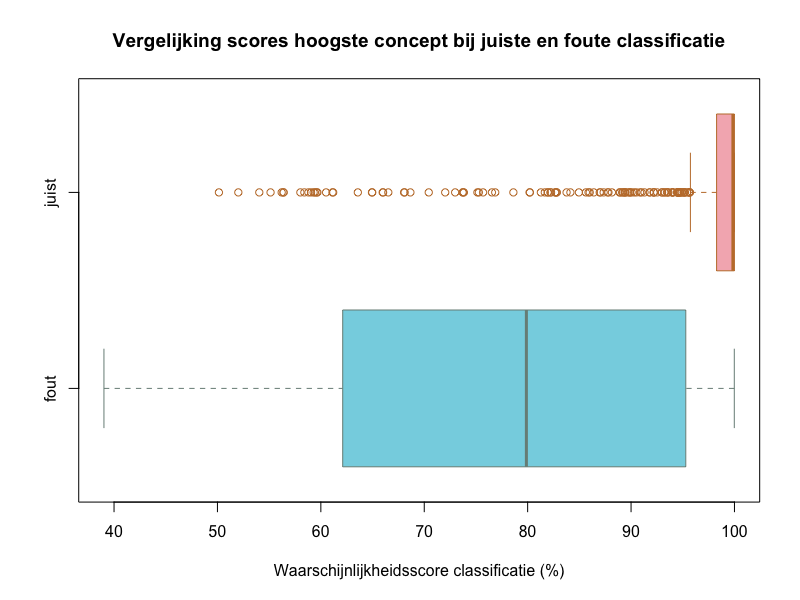
\includegraphics[width=\textwidth]
	{boxplot_hoogste_concept.png}
	\caption[Vergelijking van de waarschijnlijkheidsscores van de juiste en foute classicaties van het custom model]{Twee boxplots die de waarschijnlijkheidsscores vergelijken van het Periodemodel bij juiste en foute classificatie. In tegenstelling tot in figuur \ref{fig:boxplot-clarifai} is er geen overlapping tussen de interkwartielafstand van de foute classificaties en de boxplot van de juiste classificaties.}
	\label{fig:boxplot-tag1}
\end{figure}

\begin{table}
	\renewcommand\arraystretch{1.2}
	\centering
	\begin{tabular}{*{3}{c}}
		\toprule
		drempelwaarde (\%) & aandeel juiste classificaties (\%) & aantal foute classificaties (\%) \\
		\midrule
		95 & 87 & 3,7 \\
		[\smallskipamount]
		90 & 91 & 4,6 \\
		[\smallskipamount]
		80 & 95 & 6,6 \\
		[\smallskipamount]
		55 & 100 & 11 \\
		\bottomrule
	\end{tabular}
	\caption{Verhouding tussen drempelwaarde, totaal aantal van de juiste classificaties en het aantal foute classificaties}
	\label{tab:drempelwaarde-custom-tag1}
\end{table}

\subsection{Rekening houden met de waarschijnlijkheidsscore van de tweede tag}
Anderzijds kan er ook gekeken worden naar de waarschijnlijkheidsscore van het tweede hoogste concept dat door het model gegeven wordt. Als het model een foto correct geclassificeerd heeft, dan krijgt het tweede concept in 64\% van de gevallen een waarschijnlijkheiddscore van (afgerond) 0\%. Wanneer het model een foto fout geclassificeerd heeft, dan ligt de mediaan van de waarschijlijkheidsscore voor het tweede concept op 17\% en het gemiddelde op 19\%. Ook uit figuur \ref{fig:boxplot-tag2} blijkt dat er weinig overlapping is tussen de waarschijnlijkheidsscores van de tweede tag als de classificatie juist of fout is. Door de tags te weerhouden waarvan het tweede concept een te hoge score heeft, kunnen eveneens fouten vermeden worden. In tabel \ref{tab:drempelwaarde-custom-tag2} worden hiervoor ook enkele voorstellen gedaan.

\begin{figure}
	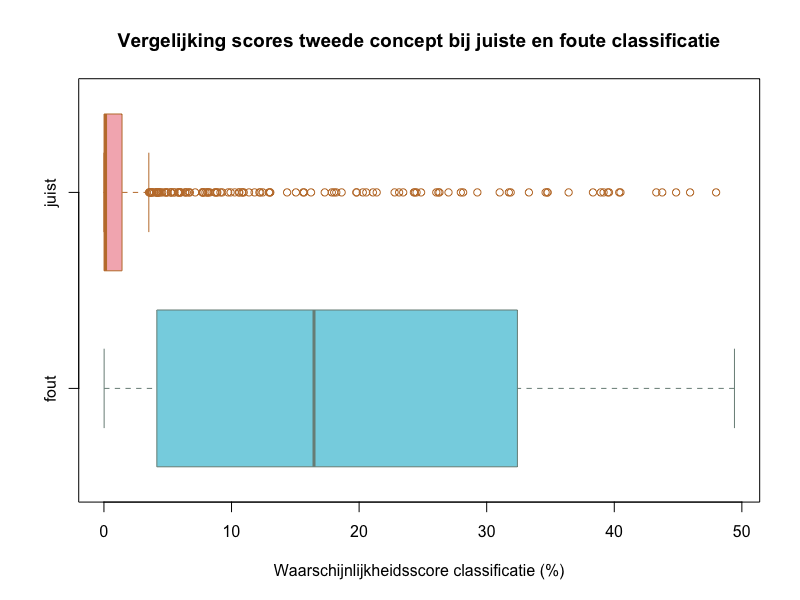
\includegraphics[width=\textwidth]
	{boxplot_tweede_concept.png}
	\caption[Vergelijking van de waarschijnlijkheidsscores van de juiste en foute classicaties van het custom model]{Twee boxplots die de waarschijnlijkheidsscores vergelijken van het tweede concept van het Periodemodel bij juiste en foute classificatie. Net als in figuur \ref{fig:boxplot-tag1} is er geen overlapping tussen de interkwartielafstanden van beide boxplots.}
	\label{fig:boxplot-tag2}
\end{figure}

\begin{table}
	\renewcommand\arraystretch{1.2}
	\centering
	\begin{tabular}{*{3}{c}}
		\toprule
		drempelwaarde (\%) & aandeel juiste classificaties (\%) & aantal foute classificaties (\%) \\
		\midrule
		5 & 87,5 & 3,3 \\
		[\smallskipamount]
		10 & 91 ,6& 4,5 \\
		[\smallskipamount]
		15 & 93,6 & 5,6 \\
		[\smallskipamount]
		48 & 100 & 12 \\
		\bottomrule
	\end{tabular}
	\caption{Verhouding tussen een drempelwaarde voor het tweede hoogste concept, totaal aandeel van de juiste tags en het aantal foute tags}
	\label{tab:drempelwaarde-custom-tag2}
\end{table}

